\chapter{Building a railway graph using EGM Dataset}

\resp{Lorenzo Rizzi}



\section{The EuroGlobalMap dataset}
 
EuroGlobalMap \cite{EGM} is a pan-European topographic database at global level of detail that provides extensive and precise territorial information including features such as waterways, road networks, and rail infrastructure. EGM utilizes Geographic Information System (GIS) data files (shapefiles, ...) to encode and represent spatial information for each type of \textit{feature} (a generic entity on the surface on Earth, in GIS jargon).

In the present work, we are going to extract data on the distribution of European railways from the EGM dataset with the purpose of building a graph representation of rail connections at large scale at a national level and across the whole Europe.
\section{Building the graph}

EGM offers a great variety of spatial information, ranging from highways to waterways. However, we are only interested in the railway infrastructure, thus we need to select the proper \textit{feature} from the database. In particular, using R package \textit{simple feature}, meant to digest shapefiles, we can easily retrieve two dataframes for each country. The first one contains spatial information (longitude, latitude) on all rail stations in the selected country. Together with longitude and latitude, a list of attributes associated with each station (high-speed, underground, national relevance) is also provided. Stations are considered $0$-dimensional, i.e. as points $p$ in the map. The second dataframe contains spatial information on railways lines. Each railway line is encoded as a \textit{linestring} object, which is essentially a pair of points $p_1, p_2$ representing the endpoints of the straight railroad. 

\paragraph{Stations analysis} Data analysis of station positions is quite straightforward. Using R, it is easy to read the initial dataframes containing geometric points and to build new dataframes with the following columns:
nodeID, nodeLabel, latitude, longitude, country\_name, country\_ISO3.

We run the analysis on the following countries: 
$$
AL, AT,BE, BG,CHLI, CY,CZ,DE,DK,EE,ES,FI,FR, GB, GE, GR ,HR, HU,IE, IS
$$
However, data on railways wasn't found in the provided folder for three countries (Albania, Iceland, Cyprus) so they will be excluded


\paragraph{Railway lines analysis} We already have the nodes of our graph, and we now need to connect these nodes. The second dataframe is composed of \textit{linestring}, i.e. pairs of spatial coordinates. Unfortunately, however, EGM does not provide direct connectivity information between stations, but only the coordinates of the endpoints of each railroad segment. Hence, we extract the endpoints of each lines from the EGM database and, by comparing distances using a spatial threshold, associate these points with the nearest railway station. If no stations is found within the spatial threshold, a placeholder is used instead (\texttt{NA} in R). By executing this procedure and mapping endpoints to known stations using a fixed threshold ($minStation$), a significant number of lines in the EGM database remain unmatched. This occurs because a single row in the EGM database (i.e., a line) typically represents only a segment of a railroad connecting two stations, and therefore some lines may have endpoints located in rural or intermediate areas. The algorithm that was used to retrieve the full edge between nodes is the following:
\begin{itemize}
	\item Fix a threshold $minStation$. For each line in the EGM database, extract its endpoints and compare them with the previously computed stations. If the distance is less than $minStation$, associate the endpoint with the corresponding station's nodeID; otherwise, assign \texttt{NA}.
	\item At the end of this procedure, some lines will have both origin and destination matched. These lines are moved to a definitive dataframe, and their two endpoints are joined as an edge in the graph.
	\item Identify \textit{downstream} segments, i.e., lines whose destination is close to a station while the origin is set to \texttt{NA} (i.e., too far from any station). Then, iterate over all non-definitive lines and search for the optimal \textit{upstream} link, defined as the nearest line (within a distance less than $minRails$) to the origin of the downstream segment. Repeat this process until a complete chain is formed, i.e., the downstream node is successfully connected to an upstream node.
\end{itemize}
An illustration of the algorithm is shown in Fig.\ref{fig:algo}. Once the edges connecting stations are found, one can write the information in a $.txt$ file and plot the results
\begin{figure}
	\centering
	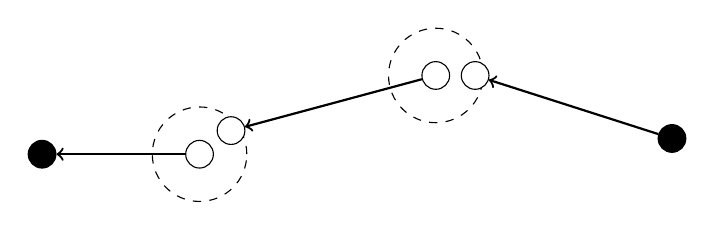
\begin{tikzpicture}[scale=1, every node/.style={circle, draw, minimum size=10pt, inner sep=0pt}]
		
		% Primo edge: orizzontale
		\node[fill=black] (A1) at (0,0) {};
		\node[fill=white] (B1) at (2,0) {};
		\draw[dashed] (B1) circle [radius=0.6];
		\draw[thick, <-] (A1) -> (B1);
		
		% Secondo edge: leggermente inclinato
		\node[fill=white] (A2) at (2.4,0.3) {};
		\node[fill=white] (B2) at (5,1) {};
		\draw[dashed] (B2) circle [radius=0.6];
		\draw[thick, <-] (A2) -- (B2);
		
		\node[fill=white] (A3) at (5.5,1) {};
		\node[fill=black] (B3) at (8,.2) {};
		\draw[thick, <-] (A3) -- (B3);
		
	\end{tikzpicture}
	\caption{\textit{An illustration of how the proposed algorithm works. Black dots represent line endpoints that are sufficiently close to a station. Starting from a downstream node (on the left), the algorithm searches for a line in the database whose destination lies within a fixed distance ($minRails$) from the origin of the current downstream segment. This procedure is iterated until a node with a matched origin (i.e., associated with a known station) is found.} }
	\label{fig:algo}
\end{figure}

\paragraph{Results}
Our algorithm relies on two tunable parameters: minStation and minRails, typically ranging between 1 and 30 km depending on the size of the country. Some results are shown in Fig.\ref{fig:Belgium}.  
Overall, the outcomes are quite satisfactory when compared to actual railway maps. However, the algorithm presents some limitations. In areas where railway lines are densely tangled (as in France), it may generate multiple redundant links or, conversely, remove valid links, resulting in disconnected segments. Another issue arises from line intersections: it may occur that railway segments intersect at locations where no station is present. In such cases, the algorithm may fail to properly follow the upstream chain, leading to station disconnections. This happens because the climbing rule illustrated in Fig.~\ref{fig:algo} selects only the nearest upstream link, potentially discarding other plausible connections. A more robust version of the algorithm should instead consider all upstream candidates within a fixed spatial threshold.


\begin{figure}
	\centering
	\includegraphics[width=0.45\linewidth]{images/BelgiumGraph.pdf}
	\includegraphics[width=0.45\linewidth]{images/BelgiumReal.pdf}
	\includegraphics[width=0.45\linewidth]{images/FranceGraph.pdf}
	\includegraphics[width=0.45\linewidth]{images/FranceReal.pdf}
	\caption{\textit{On the right, the graph of Belgium's or France's railroad network with stations as nodes ($minStation = 7 km, minRails = 7 km$ for Belgium, $minStation = 30 km, minRails = 30 km$ for France, ). On the left, the corresponding spatial rendering from EGM GIS data}}
	\label{fig:Belgium}
\end{figure}


\newpage

\section{Supplementary material}
We present here more figures like the ones in Fig.\ref{fig:Belgium} for other european countries (Fig. \ref{fig:country})

\begin{figure}
	\centering
	\includegraphics[width=0.34\linewidth]{images/FinlandGraph.pdf}
	\includegraphics[width=0.34\linewidth]{images/FinlandReal.pdf}
	\includegraphics[width=0.34\linewidth]{images/GermanyGraph.pdf}
	\includegraphics[width=0.34\linewidth]{images/GermanyReal.pdf}
	\includegraphics[width=0.34\linewidth]{images/GBGraph.pdf}
	\includegraphics[width=0.34\linewidth]{images/GBReal.pdf}
	\vspace{-5pt}
	\caption{\textit{Graphs obtained and GIS drawing for Finland, France, Germany}}
	\label{fig:country}
\end{figure}
